\subsection{The basket option with the smoothing trick as in \cite{bayersmoothing}}\label{sec:The basket option with smoothing trick without a time stepping procedure}

The third experiment that we consider is the pricing of  a European  basket call option in a Black-Scholes model. The basket is composed of $d$ assets ($d=3,8,25$) and we use the same trick of smoothing the integrand that was proposed in \cite{bayersmoothing}. In this case, the dimension of the parameter space $N=d-1$. The interpolation over the parameter space is based on the tensorized Lagrangian interpolation technique with Gaussian  points. The aim of this section is to check the performance of MISC without time stepping. The main goal is to extend this case to the time stepping framework in the next section \ref{sec:The basket option under time stepping framework}


%\newpage
\subsubsection{Results using MISC}
In table \ref{table: Complexity rates of the different experiemnts  for the basket option using BS model}, we summarize the observed  complexity rates for different tested settings for the basket example. From this table, we can check that even with the $25$ dimensional case, the complexity rate in terms of the elapsed time is at least order $1$, which is better than MC, which is $2$. Detailed plots for each case are given by figures (\ref{fig:misc_3D_Basket_1}, \ref{fig:misc_3D_Basket_2}) for $d=3$, figures (\ref{fig:misc_8D_Basket_1}, \ref{fig:misc_8D_Basket_2}) for $d=8$ and figures (\ref{fig:misc_25D_Basket_1}, \ref{fig:misc_25D_Basket_2}) for $d=25$. Mainly, from the plots, 
we checked  that we achive the prescribed tolerance using MISC, the convergence rates of mixed differences which is a basic assumption for using MISC (we observe exponential decay of error rates wrt to the number of quadrature points) and finally the complexity rates. In the next Section, we try to extend these results to the time stepping framework.


\begin{table}[h!]
	\centering
	\begin{tabular}{l*{3}{c}r}
		\# assets  \textbackslash          & $3$ & $8$ & $25$   \\
		\hline
		rate   & $-1/3$ & $-9/20$ & $-16/25$  \\
		\hline
	\end{tabular}
	\caption{Complexity rates of the different experiments  for the basket option using BS model}
	\label{table: Complexity rates of the different experiemnts  for the basket option using BS model}
\end{table}	

\subsubsection*{Case of $3$-dimensional Basket}
\begin{figure}[!h]
	\centering
	\begin{subfigure}{.4\textwidth}
		\centering
		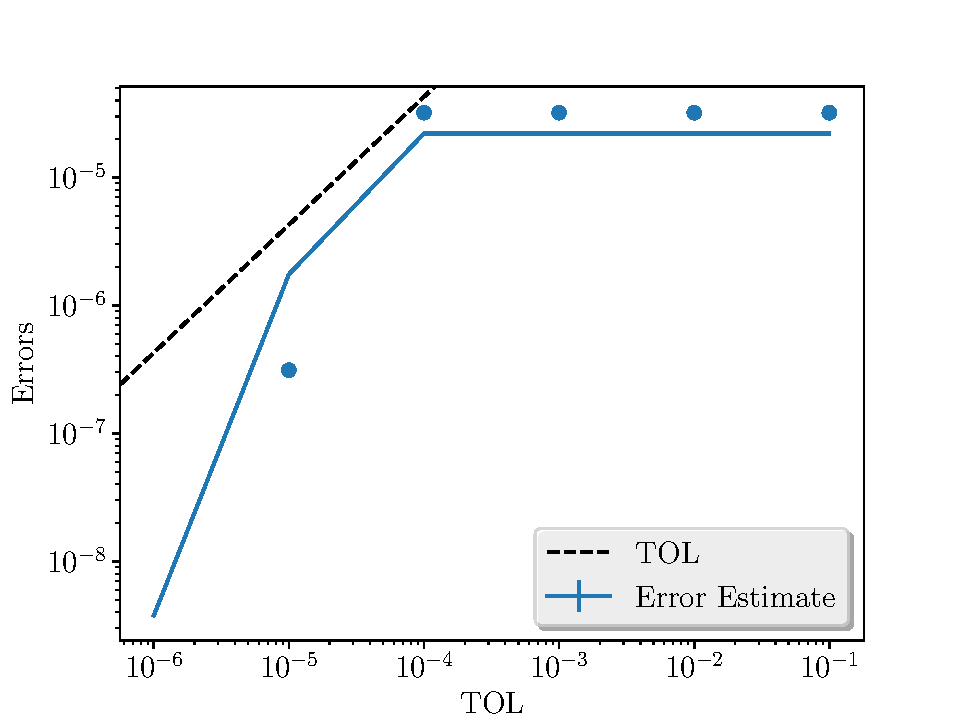
\includegraphics[width=1\linewidth]{./figures/3D_basket/error_estimate.pdf}
		\caption{Error estimate}
		\label{fig:misc_3D_Basket_sub1}
	\end{subfigure}%
	\begin{subfigure}{.4\textwidth}
		\centering
		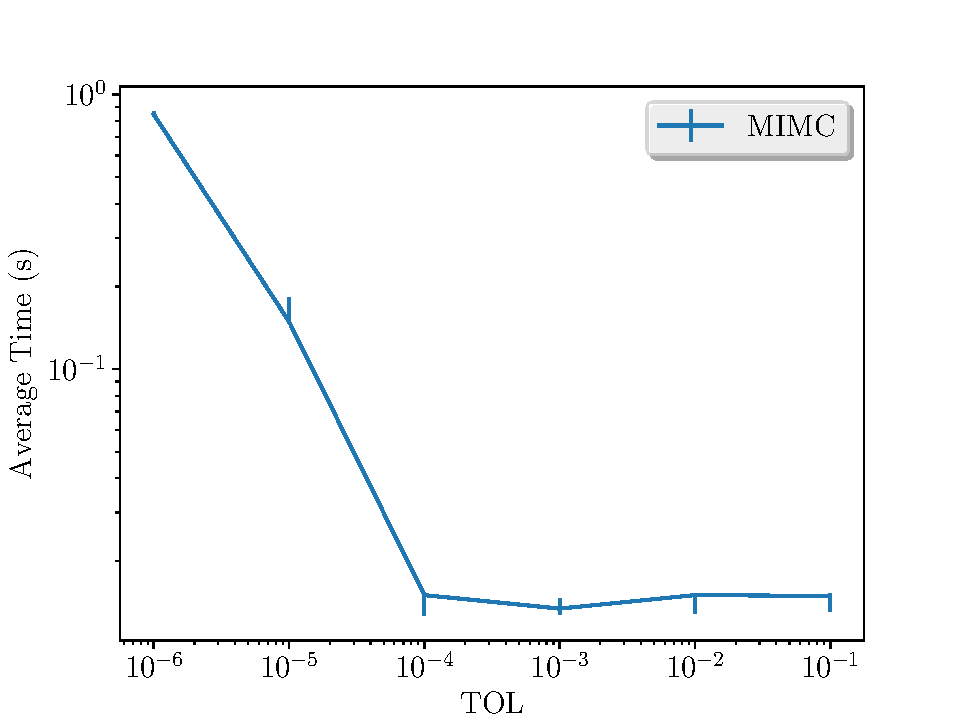
\includegraphics[width=1\linewidth]{./figures/3D_basket/average_running_time.pdf}
		\caption{Average running time as a function of $\text{TOL}$}
		\label{fig:misc_3D_Basket_sub2}
	\end{subfigure}%
	\caption{Convergence and complexity results for the $3$-dimensional basket option using BS model.}
	\label{fig:misc_3D_Basket_1}
\end{figure}



\begin{figure}[!h]
	\centering
	\begin{subfigure}{.4\textwidth}
		\centering
		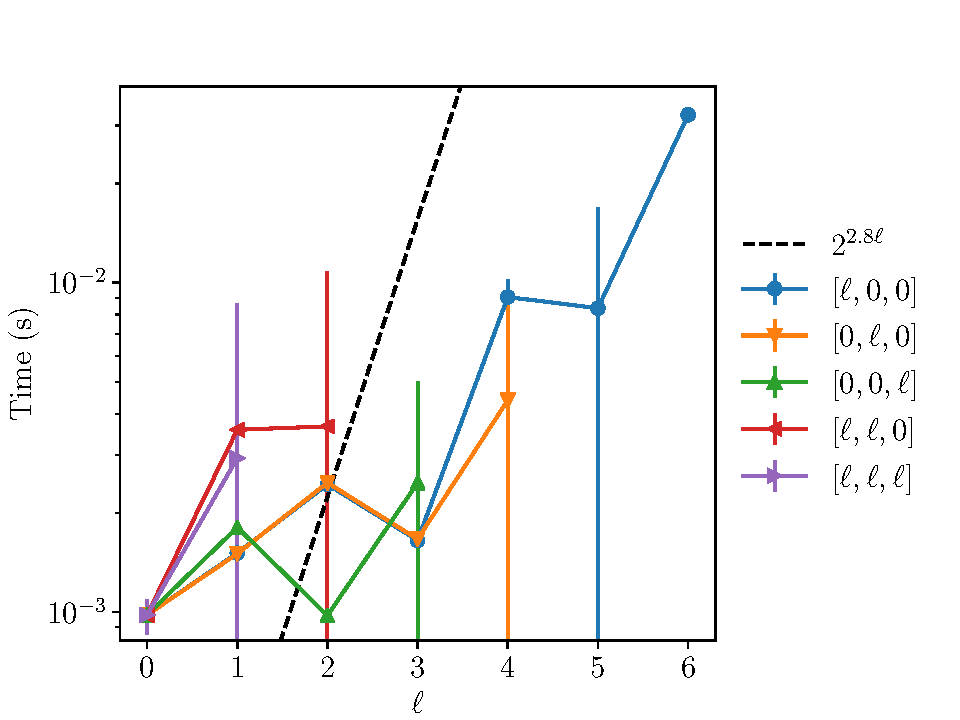
\includegraphics[width=1\linewidth]{./figures/3D_basket/level_work.pdf}
		\caption{Average Computational time per level.}
		\label{fig:misc_3D_Basket_sub3}
	\end{subfigure}%
	\begin{subfigure}{.4\textwidth}
		\centering
		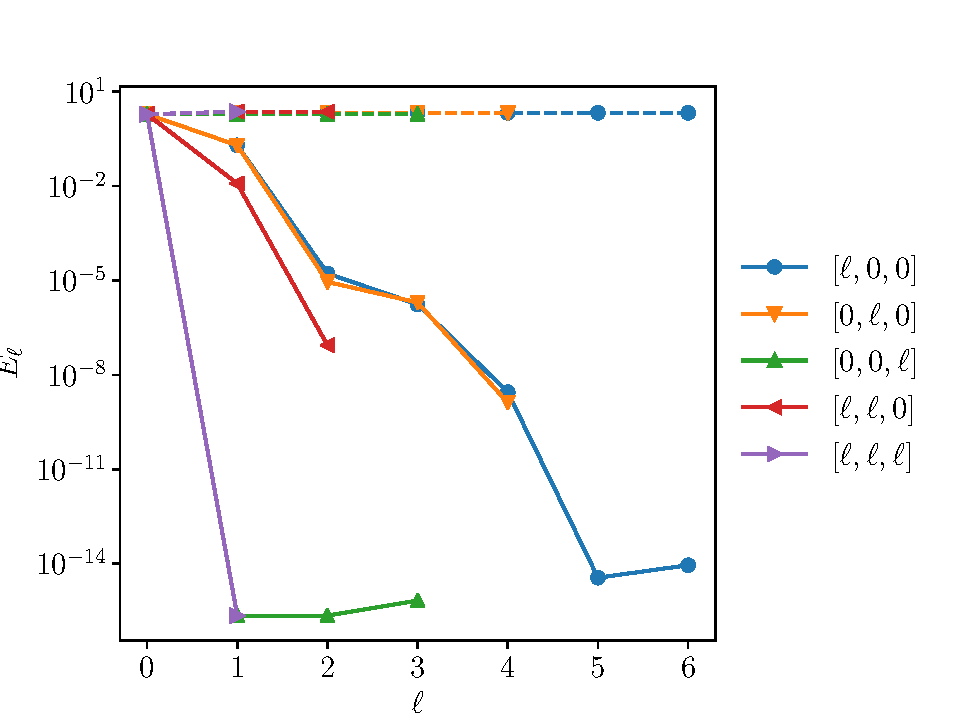
\includegraphics[width=1\linewidth]{./figures/3D_basket/levels_error_rate.pdf}
		\caption{The convergence rate of mixed differences per level.}
		\label{fig:misc_3D_Basket_sub4}
	\end{subfigure}%
	\caption{Convergence and work rates for discretization levels for the $3$-dimensional basket option using BS model.}
	\label{fig:misc_3D_Basket_2}
\end{figure}

\FloatBarrier


\subsubsection*{Case of $8$-dimensional Basket}
\begin{figure}[!h]
	\centering
	\begin{subfigure}{.4\textwidth}
		\centering
		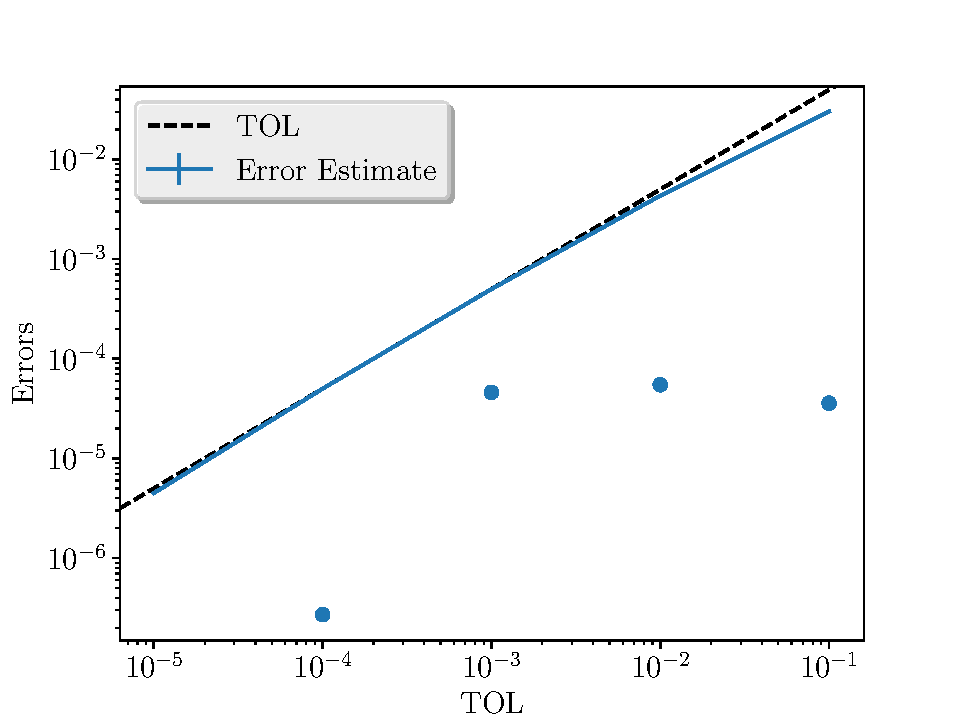
\includegraphics[width=1\linewidth]{./figures/8D_basket/error_estimate.pdf}
		\caption{Error estimate}
		\label{fig:misc_8D_Basket_sub1}
	\end{subfigure}%
	\begin{subfigure}{.4\textwidth}
		\centering
		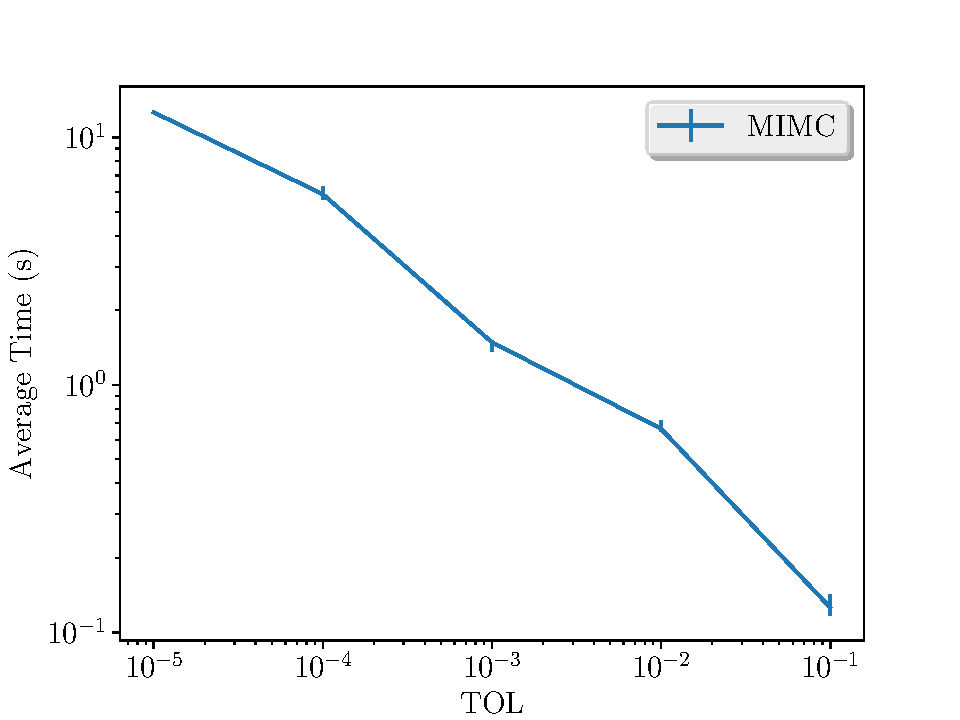
\includegraphics[width=1\linewidth]{./figures/8D_basket/average_running_time.pdf}
		\caption{Average running time as a function of $TOL$}
		\label{fig:misc_8D_Basket_sub2}
	\end{subfigure}%
	\caption{Convergence and complexity results for  the $8$-dimensional basket option using BS model.}
	\label{fig:misc_8D_Basket_1}
\end{figure}



\begin{figure}[!h]
	\centering
	\begin{subfigure}{.4\textwidth}
		\centering
		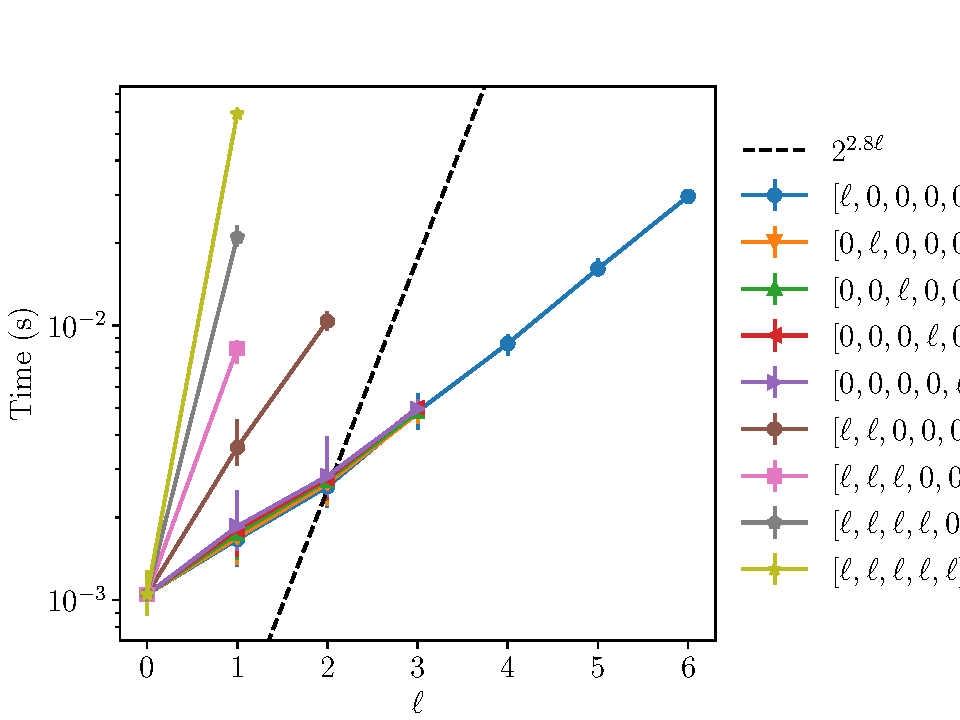
\includegraphics[width=1\linewidth]{./figures/8D_basket/level_work.pdf}
		\caption{Average Computational time per level.}
		\label{fig:misc_8D_Basket_sub3}
	\end{subfigure}%
	\begin{subfigure}{.4\textwidth}
		\centering
		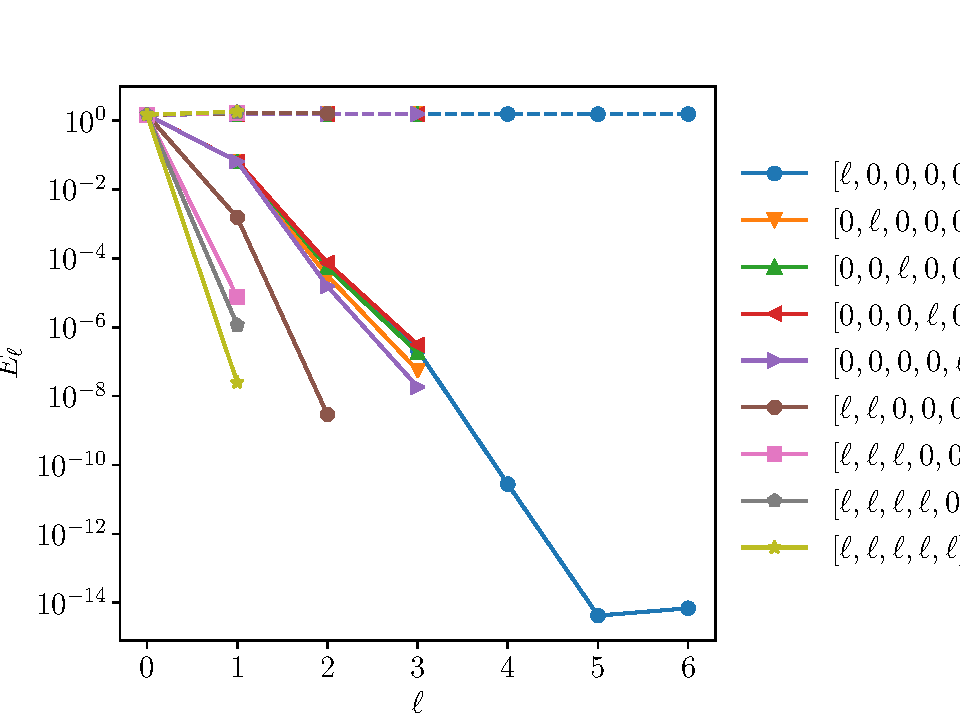
\includegraphics[width=1\linewidth]{./figures/8D_basket/levels_error_rate.pdf}
		\caption{The convergence rate of mixed differences per level.}
		\label{fig:misc_8D_Basket_sub4}
	\end{subfigure}%
	\caption{Convergence and work rates for discretization levels for the $8$-dimensional basket option using BS model.}
	\label{fig:misc_8D_Basket_2}
\end{figure}
\FloatBarrier

\subsubsection*{Case of $25$-dimensional Basket}
\begin{figure}[h!]
	\centering
	\begin{subfigure}{.4\textwidth}
		\centering
		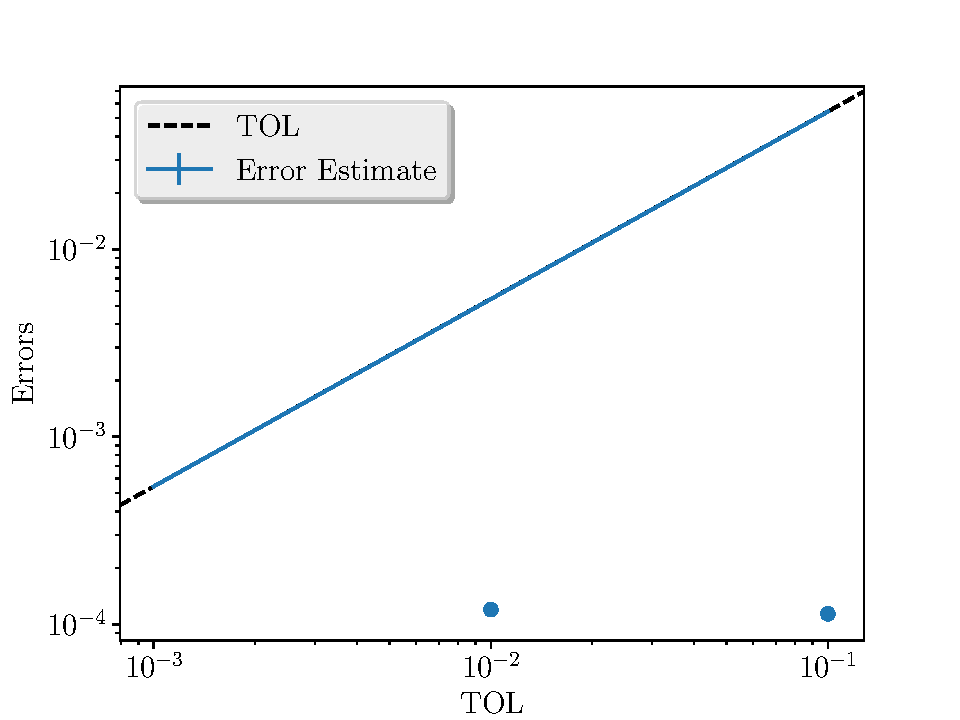
\includegraphics[width=1\linewidth]{./figures/25D_basket/error_estimate.pdf}
		\caption{Error estimate}
		\label{fig:misc_25D_Basket_sub1}
	\end{subfigure}%
	\begin{subfigure}{.4\textwidth}
		\centering
		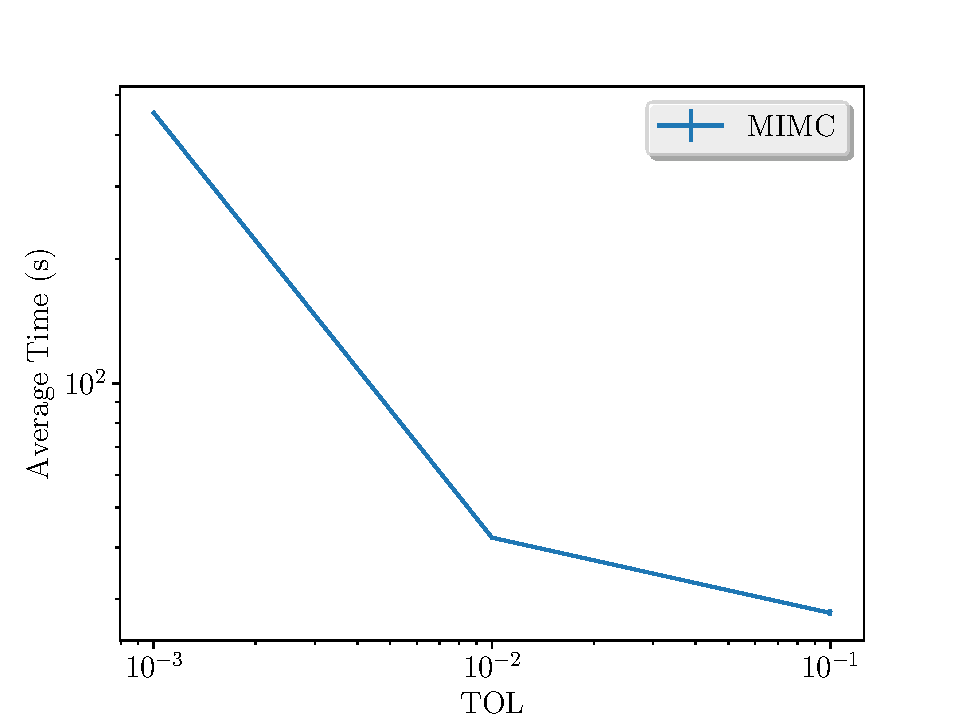
\includegraphics[width=1\linewidth]{./figures/25D_basket/average_running_time.pdf}
		\caption{Average running time as a function of $TOL$}
		\label{fig:misc_25D_Basket_sub2}
	\end{subfigure}%
	\caption{Convergence and complexity results for  the $25$-dimensional basket option using BS model.}
	\label{fig:misc_25D_Basket_1}
\end{figure}



\begin{figure}[h!]
	\centering
	\begin{subfigure}{.4\textwidth}
		\centering
		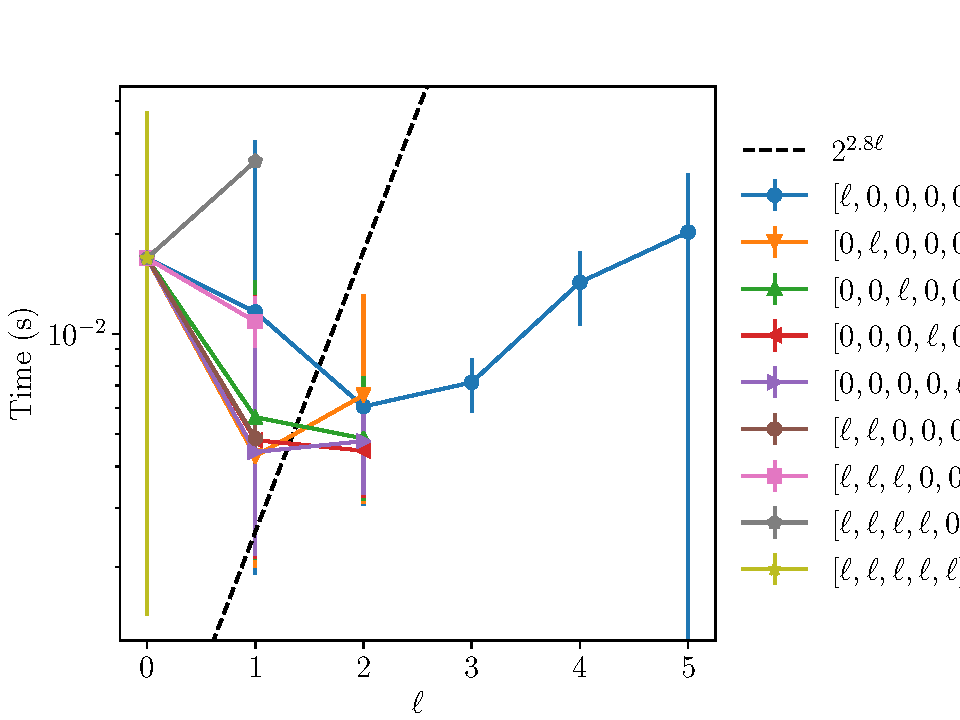
\includegraphics[width=1\linewidth]{./figures/25D_basket/level_work.pdf}
		\caption{Average Computational time per level.}
		\label{fig:misc_25D_Basket_sub3}
	\end{subfigure}%
	\begin{subfigure}{.4\textwidth}
		\centering
		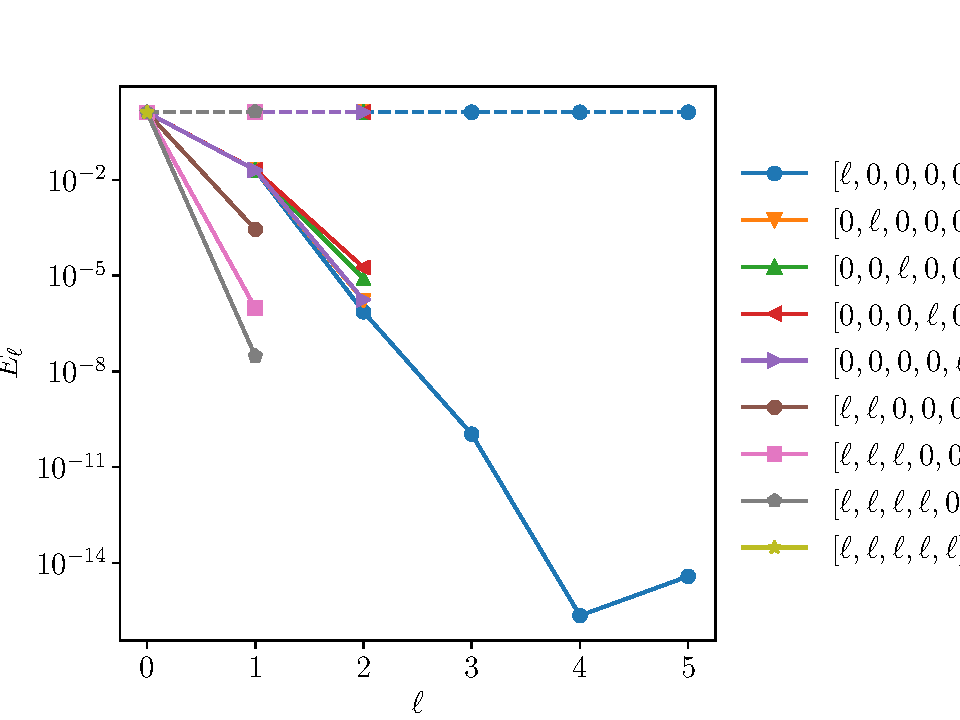
\includegraphics[width=1\linewidth]{./figures/25D_basket/levels_error_rate.pdf}
		\caption{The convergence rate of mixed differences per level.}
		\label{fig:misc_25D_Basket_sub4}
	\end{subfigure}%
	\caption{Convergence and work rates for discretization levels for the $25$-dimensional basket option using BS model.}
	\label{fig:misc_25D_Basket_2}
\end{figure}


\FloatBarrier 